% !TEX root = /media/ueslei/Ueslei/INPE/PCI/Guia_COAWST/main.tex
\chapterimage{ocean2.jpg}
\chapter{Construindo o SWAN}

\noindent O SWAN utiliza os arquivos com extensão \textit{.bot} e \textit{.grd} para suas simulações. Neste caso, criaremos eles a partir da grade do ROMS, porém sem introduzir dados iniciais, pois como ele rodará acoplado, apenas alguns dias de simulação são o suficiente para que o modelo estabilize e envie as troca de informação entre os modelos ocorra normalmente.
\bigskip

\noindent Neste caso,  utilize o script do MATLAB \textit{make\_swan.m} que está dentro da pasta de repositório:
\bigskip

\begin{bashcode}
/home/nome.sobrenome/repositorio/SWAN_scripts
\end{bashcode}
\bigskip

\noindent Conforme a Figura \textcolor{bleu_cite}{\ref{makeswan}}, o script possui a seguinte construção:
\bigskip

\begin{figure}[H]
    \centering
    \captionsetup{justification=centering}
    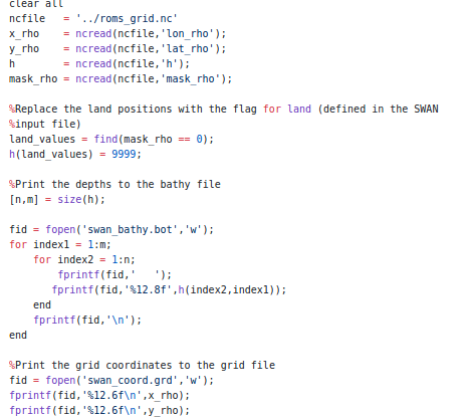
\includegraphics[width=0.47\textwidth]{makeswan.png}
    \caption{O script \textit{make\_swan.m}.}
    \label{makeswan}
\end{figure}
\bigskip

\noindent Para gerar os dois arquivos do SWAN, procure no script a variável \textit{ncfile} e altere o diretório para o caminho onde está sua grade do ROMS.
\bigskip

\noindent Execute o script e serão criados os dois arquivos: \textit {swan\_coord.grd} e \textit{swan\_bathy.bot}. Os dois arquivos deverão ser colocados dentro da sua pasta de projetos.
